% !TEX TS-program = xelatex
%
% Created by Chris on 2020-07-19.
% Copyright (c) Chris von Csefalvay, 2020.
\documentclass{article}
\usepackage{amsmath}
\usepackage{polyglossia}
\usepackage{hyperref}

% Bibliography styling
\usepackage[super,square,sort&compress,numbers]{natbib}
\bibliographystyle{unsrtnat}
\usepackage{url}
\urlstyle{same}

% Language and hyphenation
% \usepackage[english]{babel}
\usepackage[htt]{hyphenat}

% Graphics
\usepackage{graphicx}

\hypersetup
{
  pdftitle   = {A differential game analysis of social distancing in COVID-19},
  pdfauthor  = {Chris von Csefalvay}
}

\title{A differential game analysis of social distancing in COVID-19}
\author{Chris von Csefalvay}

\begin{document}

\maketitle

\begin{abstract}
    Abstract
\end{abstract}

\section{Introduction} % (fold)
\label{sec:introduction}
Where an infectious disease is not amenable to population-level prevention through vaccination and risks are non-trivial, non-pharmaceutical interventions (NPIs) remain the principal tool of public health to respond to an outbreak. This is the case with novel infectious diseases that have no specific treatment and no prophylactic (vaccine) available. In the absence of pharmaceutical interventions of proven effectiveness, in particular prophylactically, the main public health response to the emerging pandemic of COVID-19, a viral syndrome caused by the (+)ssRNA virus SARS-CoV-2 (order \emph{Nidovirales}, family \emph{Coronaviridae}, genus \emph{Betacoronavirus}, subgenus \emph{Sarbecovirus}), has rested principally on NPIs, first and foremost social distancing and ancillary steps intended to facilitate that.

In general, any course of conduct that reduces the encounter rate between an individual and other individuals can be considered a form of social distancing. This may be brought about through limiting public facilities for such encounters ('lockdowns'), through limiting individual gatherings by size ('large-gathering bans') and through encouraging individual social distancing. From the perspective of game theory, social distancing can be viewed as a non-cooperative game of a population $P_{1 \ldot n}$ of size $n$, where at any given time $t \in [t_0, t_{e}]$, the strategy adopted by $p_i$ is denoted as $\sigma (p_i, t)$. For the sake of simplicity, we assume that distancing is either not exercised at all or perfectly exercised, i.e. $\sigma (p_i, t) \in \{ 0, 1 \}$. Then, for the entire population, the overall strategy can be described as 

\begin{equation}
	\bar{\sigma}(P, t) = \frac{\displaystyle \sum_{i = 0}^n \sigma(p_i, t)}{n}
	\label{eq:overall_strategy}
\end{equation}

\noindent and for the entire time period, from $t_0$ to the endpoint $t_e$ (which may be eradication, elimination, natural extinction of the pathogen, the availability of a vaccine or a combination thereof), for discrete time $t$,

\begin{equation}
	\bar{\bar{\sigma}}(P) = \frac{\displaystyle \sum_{i = 0}^n \displaystyle \sum_{j = 0}^{t_e - t_0} \sigma(p_i, j)}{n (t_e - t_0)}
	\label{eq:overall_strategy_over_time}
\end{equation}

However, with each course of conduct, there is associated a cost $J(\sigma)$. For simplicity's sake, let us consider these costs to be governed by the following three precepts given a pathogen with fixed characteristics ($R_0$, transmission potential, risks \&c.). Let $\bar{\delta}(P)$ equal the proportion of persons $p \in P$ adopting strategy $\sigma_{\delta}$. It then holds that: 

\begin{enumerate}
	\item A person $p_i \in P$ opting for strategy $\delta$ (social distancing) will incur $c_d$, the immediate costs of distancing. These may be social (lessened social interaction), psychological (lessened access to support systems), economic (lower access to facilities to earn) or simple matters of convenience (access to amenities). While $c_d$ is somewhat dependent on $\bar{\bar{(P)}}$ (thus not distancing does not yield a benefit to a lone social distancer in terms of access to amenities if all of the latter are closed), it can be assumed to be largely constant.
	\item Compared to a person opting for strategy $\delta$, a person $p_i \in P$ opting for strategy $\lnot \delta$ will incur a relative additional risk $f_r(\bar{\delta}(P), t)$, i.e. contingent on the population's behaviour at time $t$.
	\item Finally, a person $p_i \in P$ will regardless of their individual choice (at least at non-trivial population sizes) gain a protective benefit, which is a function of the population's adherence to social distancing. We will denote this term as $f_c(\bar{\delta}(P), t)$.
\end{enumerate}

Then, assigning the variable $c_s$ to represent the cost of illness (economic loss, medical costs, long-term health risks), we can express the cost functions of each strategy, $\sigma_{\delta}$ (social distancing) and $\sigma_{\lnot \delta}$ (no social distancing), as

\begin{equation}
	J_{\sigma_{\delta}}(p_i, t) = c_d - f_c(\bar{\delta}(P), t)
\end{equation}

\noindent and

\begin{equation}
	J_{\sigma_{\lnot \delta}}(p_i, t) = f_r(\bar{\delta}(P), t) c_s - f_c(\bar{\delta}(P), t)
\end{equation}

\noindent And consequently, it holds for the population level cost $\bar{J}$ at time $t$ that

\begin{equation}
	\bar{J}(P, t) = \frac{\displaystyle \sum_{i=0}^{\delta(P) n} J_{\sigma_{\delta}}(p_i, t) + \displaystyle \sum_{j=0}^{1-\delta(P) n} J_{\sigma_{\lnot \delta}}(p_j, t)}{n}
	\label{eq:cost_eqn}
\end{equation}

\noindent and for a population over time $t_0$ to $t_e$, 

\begin{equation}
	\bar{\bar{J}}(P) = \int_{t_0}^{t_e} \bar{J}(P, t) dt
\end{equation}

As Reluga (2010) notes, the effect of social distancing diminishes with the increase in participants, the phenomenon of diminishing returns.\cite{reluga2010game} Thus, as the number of individuals in $P$ opting for social distancing increases, the marginal increase by another social distancer diminishes. This can be represented by a discount factor $h$, to yield

\begin{equation}
	\bar{J}(P) = \int_{t_0}^{t_e} e^{-ht} \frac{\delta(P) J_{\sigma_{\delta}}(P, t) + (1 - \delta(P)) J_{\sigma_{\lnot \delta}}(P, t)}{n}
\end{equation}

However, because individual decisions affect the overall gain (due to the component dependent on $\delta(P, t)$), our principal concern is not with individual action but with analysis of such strategies on a population level. This paper will in the following conceptualise infectious disease in a population as a differential game over a differential equation form of the compartmental model first described by Kermack and McKendrick\cite{kermack1927contribution} and, since its publication in 1927, widely adapted and adopted.\cite{vstvepan2007kermack,roberts1999kermack,capasso1978generalization}

% section introduction (end)

\section{Methods} % (fold)
\label{sec:methods}

\subsection{The ordinary differential equations of disease dynamics} % (fold)
\label{sub:the_ordinary_differential_equations_of_disease_dynamics}

Given a population of $n$ under the assumption that reinfection is impossible (as, e.g., in the case of measles) or rare (as is the case for SARS-CoV-2\cite{edridge2020human,deng2020primary,bao2020reinfection}), and neglecting for the time being the vital dynamics (birth, unrelated death, migration) of the population, the dynamics of any population can be modelled as a system of ordinary differential equations

\begin{equation}
	\begin{aligned}
		\frac{dS}{dt} = - \frac{\beta S I}{n} 								\\
		\frac{dI}{dt} = \frac{\beta S I}{n} - \gamma I 						\\
		\frac{dR}{dt} = \gamma I
	\end{aligned}
	\label{eq:sir_equation}
\end{equation}

\noindent under the assumption of $S + I + R = 0$, where $S$ represents susceptible individuals, $I$ represents infected/infectious individuals and $R$ accounts for removed individuals (mortality and recovery to immunity). Even in the absence of firm evidence as to whether SARS-CoV-2 infection followed by recovery would engender lifelong immunity or not,\cite{roy2020covid,ota2020will,lin2020duration} it can be assumed in the short term -- based on evidence from MERS-CoV and SARS-CoV -- that in the short term, survivors remain immune,\cite{prompetchara2020immune} and consequently the number of individuals in $R$ does not decrease.

For a population $P$ of size $n$ that pursues the population-level aggregate of strategies described by $\bar{\sigma(P)}$, the dynamics described above in Equation~\eqref{eq:sir_equation} becomes

\begin{equation}
	\begin{aligned}
		\frac{dS}{dt} = - \bar{\sigma}(P) \frac{\beta S I}{n} 				\\
		\frac{dI}{dt} = \bar{\sigma}(P) \frac{\beta S I}{n} - \gamma I 		\\
		\frac{dR}{dt} = \gamma I
	\end{aligned}
	\label{eq:sir_strat_equation}
\end{equation}

\begin{figure}
	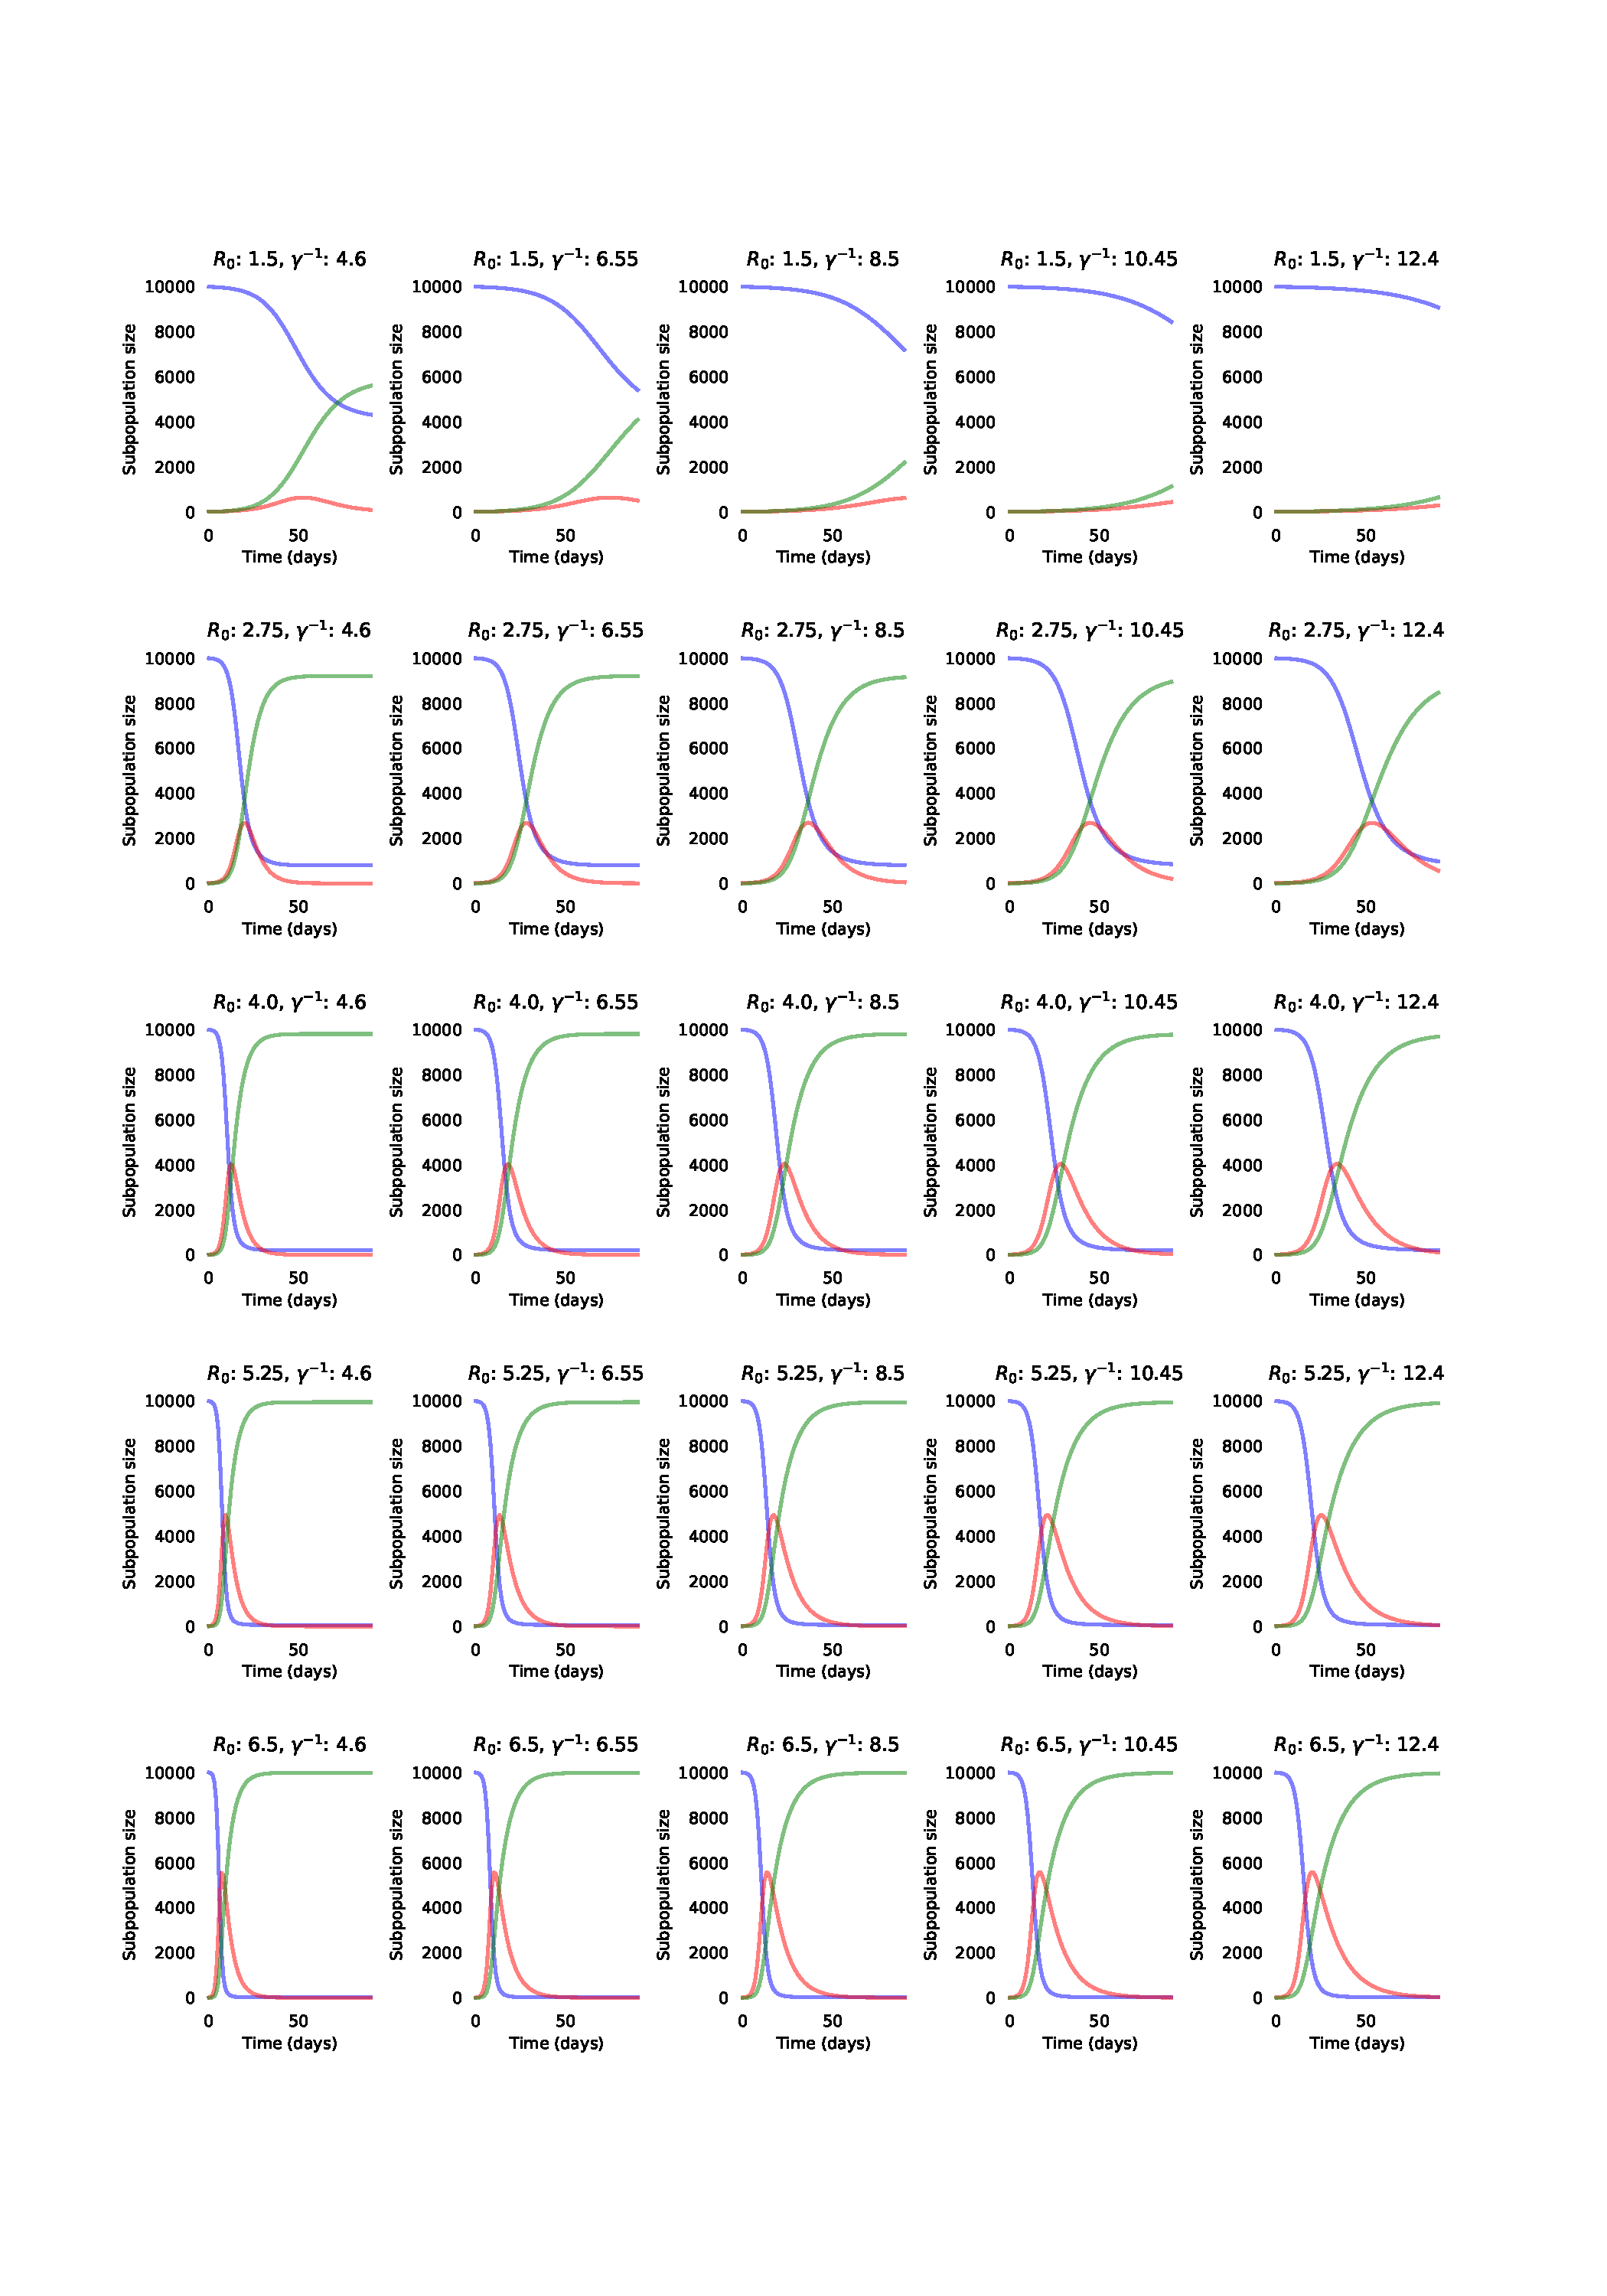
\includegraphics[width=\linewidth]{figures/fig1-odes}
	\caption{Some quantitative solutions for the SIR model's population dynamics over values of $R_0$ between 1.5 and 6.5, and values of $\gamma$ between $1/4.6$ and $1/12.4$ over a base population of 10,000 and a seed population of 1\% infected initially. For each plot, $\beta$ is inferred from an $R_0$ value of 2.67, based on Liu et al. (2020),\cite{liu2020reproductive} and the $\gamma$ parameter. The susceptible population is displayed in blue, while infected/infectious cases are marked in red and recovered cases in green.}
	\label{fig:ode_solutions}
\end{figure}

The fraction $\frac{\beta n}{\gamma}$ equals the basic reproduction number, $R_0$. For SARS-CoV-2, estimates of $R_0$ range from 1.4 to 6.49, with studies that relied on statistical estimation of $R_0$ ranging from 2.20 to 3.58, with an average of 2.67\cite{liu2020reproductive} $\gamma$, on the other hand, can be estimated as the invers of the number of days of illness, which can be approximated as $8.5 \pm 3.9$ days.\cite{pan2020clinical,liu2020risk} Figure~\ref{fig:ode_solutions} describes some analytical solutions for the differential equations of Equation~\eqref{eq:sir_equation} over a range of plausible values of $R_0$ and $\gamma$ under the assumption of an $R_0$ of 2.67.

% subsection the_ordinary_differential_equations_of_disease_dynamics (end)

\subsection{Population strategy contingent solutions to population dynamics} % (fold)
\label{sub:population_strategy_contingent_solutions_to_population_dynamics}


\begin{figure}
	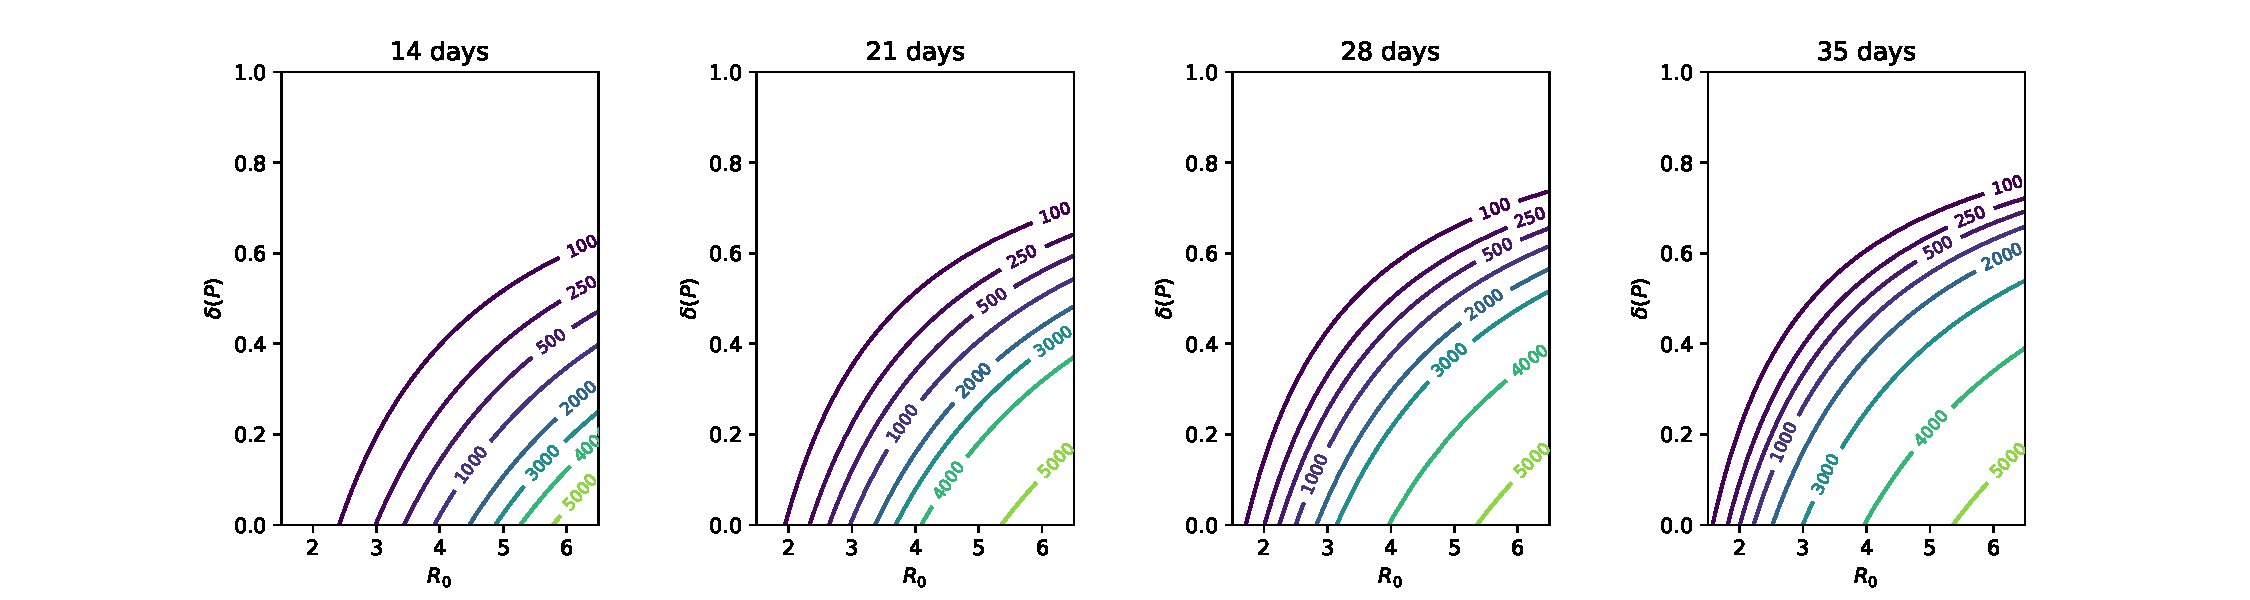
\includegraphics[width=\linewidth]{figures/fig2-strategy_solutions_by_days}
	\caption{A first naive approximation of population strategy contingent dynamics in a population of 10,000 with an initial seed population of 1\% infected initially, showing the maximum number of infected by 14, 21, 28 and 35 days. For each plot, the $\gamma$ parameter was estimated to be $\frac{1}{8.5}$, based on Pan et al. (2020) and Liu et al. (2020),\cite{pan2020clinical,liu2020risk}. This initial approach assumes a constant effect to social distancing, i.e. not accounting for diminishing returns, whether over time or over population participating in social distancing.}
	\label{fig:first_naive_solution}
\end{figure}

Let us now draw on Equation~\eqref{eq:overall_strategy} to adjust the system of differential equations in Equation~\eqref{eq:sir_equation}. A population $P$ adopting the overall strategy $\bar{\sigma}(P, t)$ at time $t$ will have an efficiency factor of $\delta(P, t)$, bounded by $[0; 1]$, where

\begin{equation}
	\begin{aligned}
		\delta(P, t) = \frac{\displaystyle \sum_{i = 1}^n \sigma(p_i, t)}{n}
	\end{aligned}
	\label{eq:delta_p_t}
\end{equation} 

\noindent in other words, $\delta(P, t)$ is the fraction of the population $P$ that is engaged in social distancing at time $t$. An initial naive approximation of the effect of various values of $\delta(P, t)$ (as a rough proxy of $\bar{\sigma{(P, t)}}$) is represented by Figure~\ref{fig:first_naive_solution}. This does not, however, account for the underlying differential game, i.e. the individual and societal cost of distancing or not distancing. In the following refinement of the model, we will consider each of these in turn.

% subsection population_strategy_contingent_solutions_to_population_dynamics (end)

\subsection{Cost and strategy} % (fold)
\label{sub:cost_and_strategy}

For each member $p$ of the population $P$, there exists a cost function of distancing $J_{\delta}(P, t)$ for any given time $t$ contingent on the population $P$'s behaviour, and a corresponding function $J_{\lnot \delta}(P, t)$ for not distancing (see Equation~\eqref{eq:cost_eqn}). As noted above, three major factors govern the cost for each individual: the cost of distancing per unit time ($c_d$, comprising economic and non-economic costs of social distancing), the risk of contracting the disease ($f_r(\bar{\delta}(P), t)$) and the cost of sickness per unit time spent sick ($c_s$). The cost is decreased by the social benefit of distancing, which is, at least outside trivially sized populations, largely independent from the individual and depends on how many in the population are engaging in social distancing ($f_c(\bar{\delta}(P), t)$).

For a population of rational actors, it can be assumed that they will adopt the strategy that is the most beneficial given the information they have. It deserves mention that, as Reluga (2006) alludes to, decisions are made by players based on the information they have,\cite{reluga2006evolving} which may often be incomplete or even outright false: perceptions, not necessarily reality, drive decision-making. Ignoring the social benefit, the equilibrium point between strategies, $J_{\delta}(P, t) = J_{\lnot \delta}(P, t)$ is reached for the equilibrium condition where

\begin{equation}
	c_d = f_r(\bar{\delta}(P), t) c_s
	\label{eq:cost_risk}
\end{equation}

\noindent -- or in other words, where the cost of distancing equals the risk of contracting the disease (given the population's state) and the cost of the disease. This point also represents a subgame perfect Nash equilibrium for the underlying differential game. This is easy to see: given this equilibrium point, a person who is not socially distancing may switch to the strategy of social distancing, but would incur an unwarranted cost. Similarly, a person who is socially distancing at this time would risk more than the costs avoided by forgoing social distancing. 

\begin{figure}
	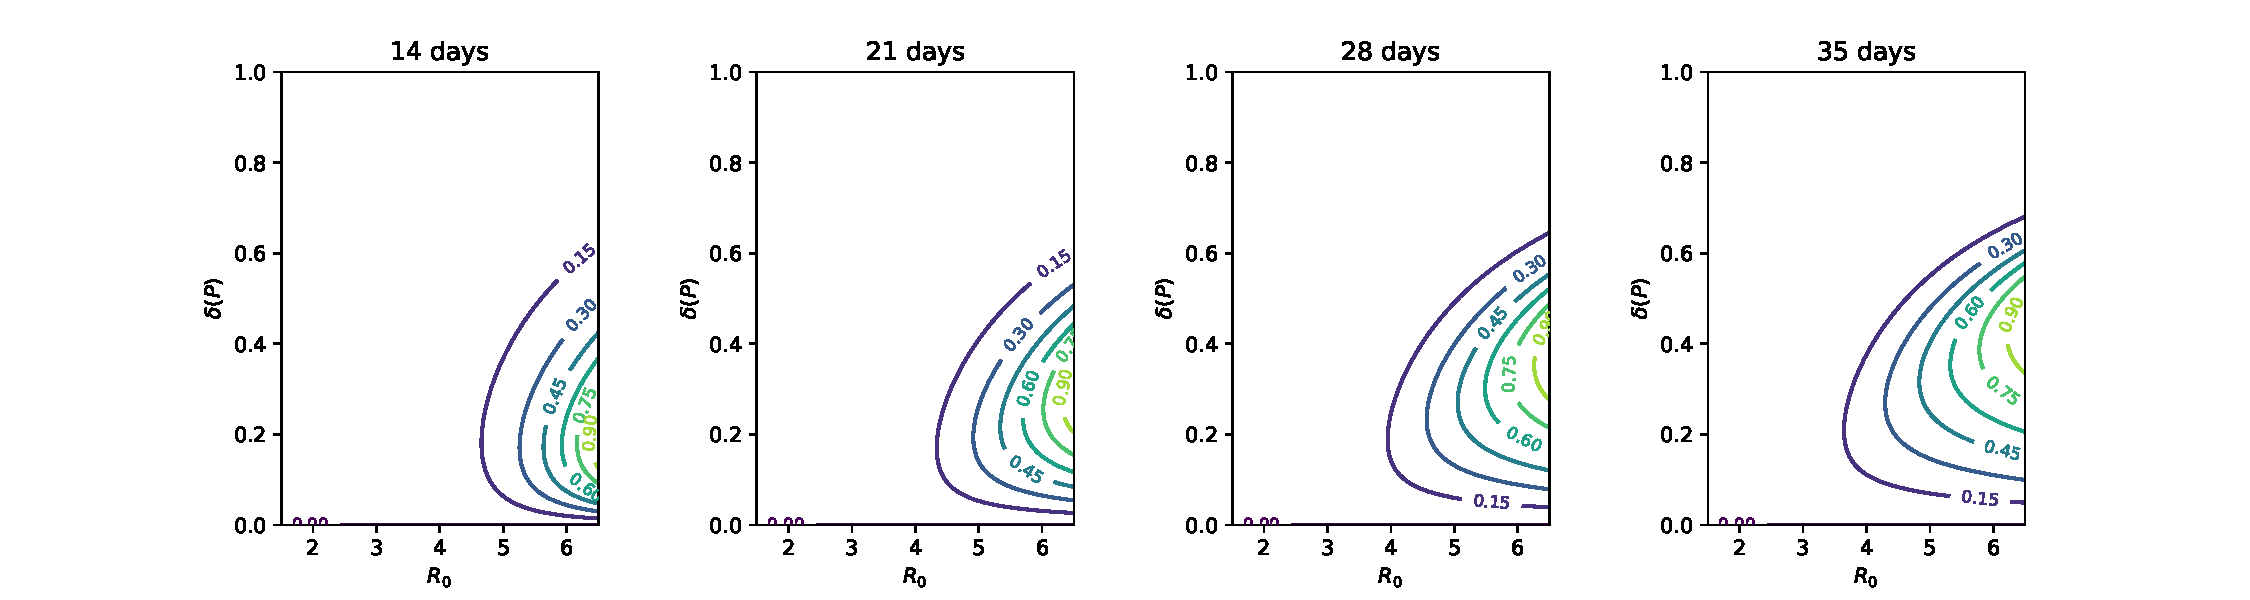
\includegraphics[width=\linewidth]{figures/fig3-risk-of-adherence}
	\caption{Relative benefits of social distancing as a function of $R_0$ and societal adherence for a population of 10,000 with an initial infected seed population of 1\%. Benefits are normalised to 1.0 against the maximum value. For each plot, the $\gamma$ parameter was estimated to be $\frac{1}{8.5}$, based on Pan et al. (2020) and Liu et al. (2020),\cite{pan2020clinical,liu2020risk}. As the plot indicates, social distancing is most effective for higher $R_0$ and mediocre overall social distancing within the population, contradicting the widely shared popular perception that social distancing is useless unless practised by an overwhelming majority and supporting the case for social distancing for all individuals.}
	\label{fig:risk_and_compliance}
\end{figure}


It is clear that the risk of disease at time $t$, $f_r(\bar{\delta}(P), t)$, is in fact reflective of the adjusted force of infection subject to the share of the population engaged in social distancing, described by $\bar{\delta}(P)$. The force of infection $\lambda$ is typically defined as $\frac{\beta I}{n}$. When adjusting for the risk of disease to an individual considering the population's response, encapsulated in $\bar{\delta}(P)$, we get

\begin{equation}
	f_r(\bar{\delta}(P), t) = \frac{\bar{\delta}(P) \beta I(t)}{n}
	\label{eq:adjusted_force_of_infection}
\end{equation}

\noindent and substituting $R_0 = \frac{\beta n}{\gamma}$ into Equation~\eqref{eq:adjusted_force_of_infection} allows us to express this as 

\begin{equation}
	f_r(\bar{\delta}(P), t) = \frac{\bar{\delta}(P) R_0 \gamma I(t)}{n^2}
	\label{eq:expanded_cost_fx}
\end{equation}

This can be solved using quantitative methods (see Figure~\ref{fig:risk_and_compliance}) to yield isorisk curves based on $R_0$ and $\delta(P)$, i.e. on pathogen-intrinsic and population-intrinsic characteristics, over time.

% subsection cost_and_strategy (end)

\subsection{Cost-risk equilibria} % (fold)
\label{sub:cost_risk_equilibria}

As noted in Equation~\eqref{eq:cost_risk}, on a social level, the equilibrium state is defined where the cost of disease times the risk of disease equals the cost of avoidance. By substituting Equation~\eqref{eq:expanded_cost_fx} into Equation~\eqref{eq:cost_risk}, we get the equilibrium equation

\begin{equation}
	c_d(t) = c_s(t) \frac{\bar{\delta}(P(t)) R_0 \gamma I(t)}{n^2}
\end{equation}

\noindent or, reformulated, 

\begin{equation}
	\frac{c_d(t)}{c_s(t)} = \frac{\bar{\delta}(P(t)) R_0 \gamma I(t)}{n^2}
\end{equation}

Expressed over the entire duration $t_{0 \ldots e}$, the cost ratio of distancing ($c_d$) and sickness ($c_s$) is

\begin{equation}
	\frac{c_d}{c_t} = \int_{t_0}^{t_e} \frac{\bar{\delta}(P(t)) R_0 \gamma I(t)}{n^2} dt
\end{equation}

% subsection cost_risk_equilibria (end)

% section methods (end)

\section{Results} % (fold)
\label{sec:results}




This risk, viewed as a function of $R_0$ and $\delta(P)$ in Figure~\ref{fig:risk_and_compliance}, indicates the somewhat counterintuitive finding that social distancing becomes more, 


% section results (end)

\bibliography{bibliography}

\end{document}
